%==========================================================================

\begin{frame}[fragile]

  {\Huge General Enhancements}

  \vspace{10pt}

\end{frame}

\begin{frame}[fragile]{General Enhancements I}
  \begin{itemize}
    \item Enable ScatterView contribute into a View that is a rvalue
    \begin{itemize}
      \item \begin{code}[keywords={}]
Experimental::contribute(subview(2d_view, ALL(), 0), scatterview);
      \end{code}
    \end{itemize}
    \item Use \texttt{Array::size\_type} for subscript operators
    \item Implement \texttt{StaticBatchSize} for HIP backend
    \item Improve \texttt{deep\_copy} performance for scalar view fill using \texttt{StaticBatchSize}
  \end{itemize}
\begin{center}
  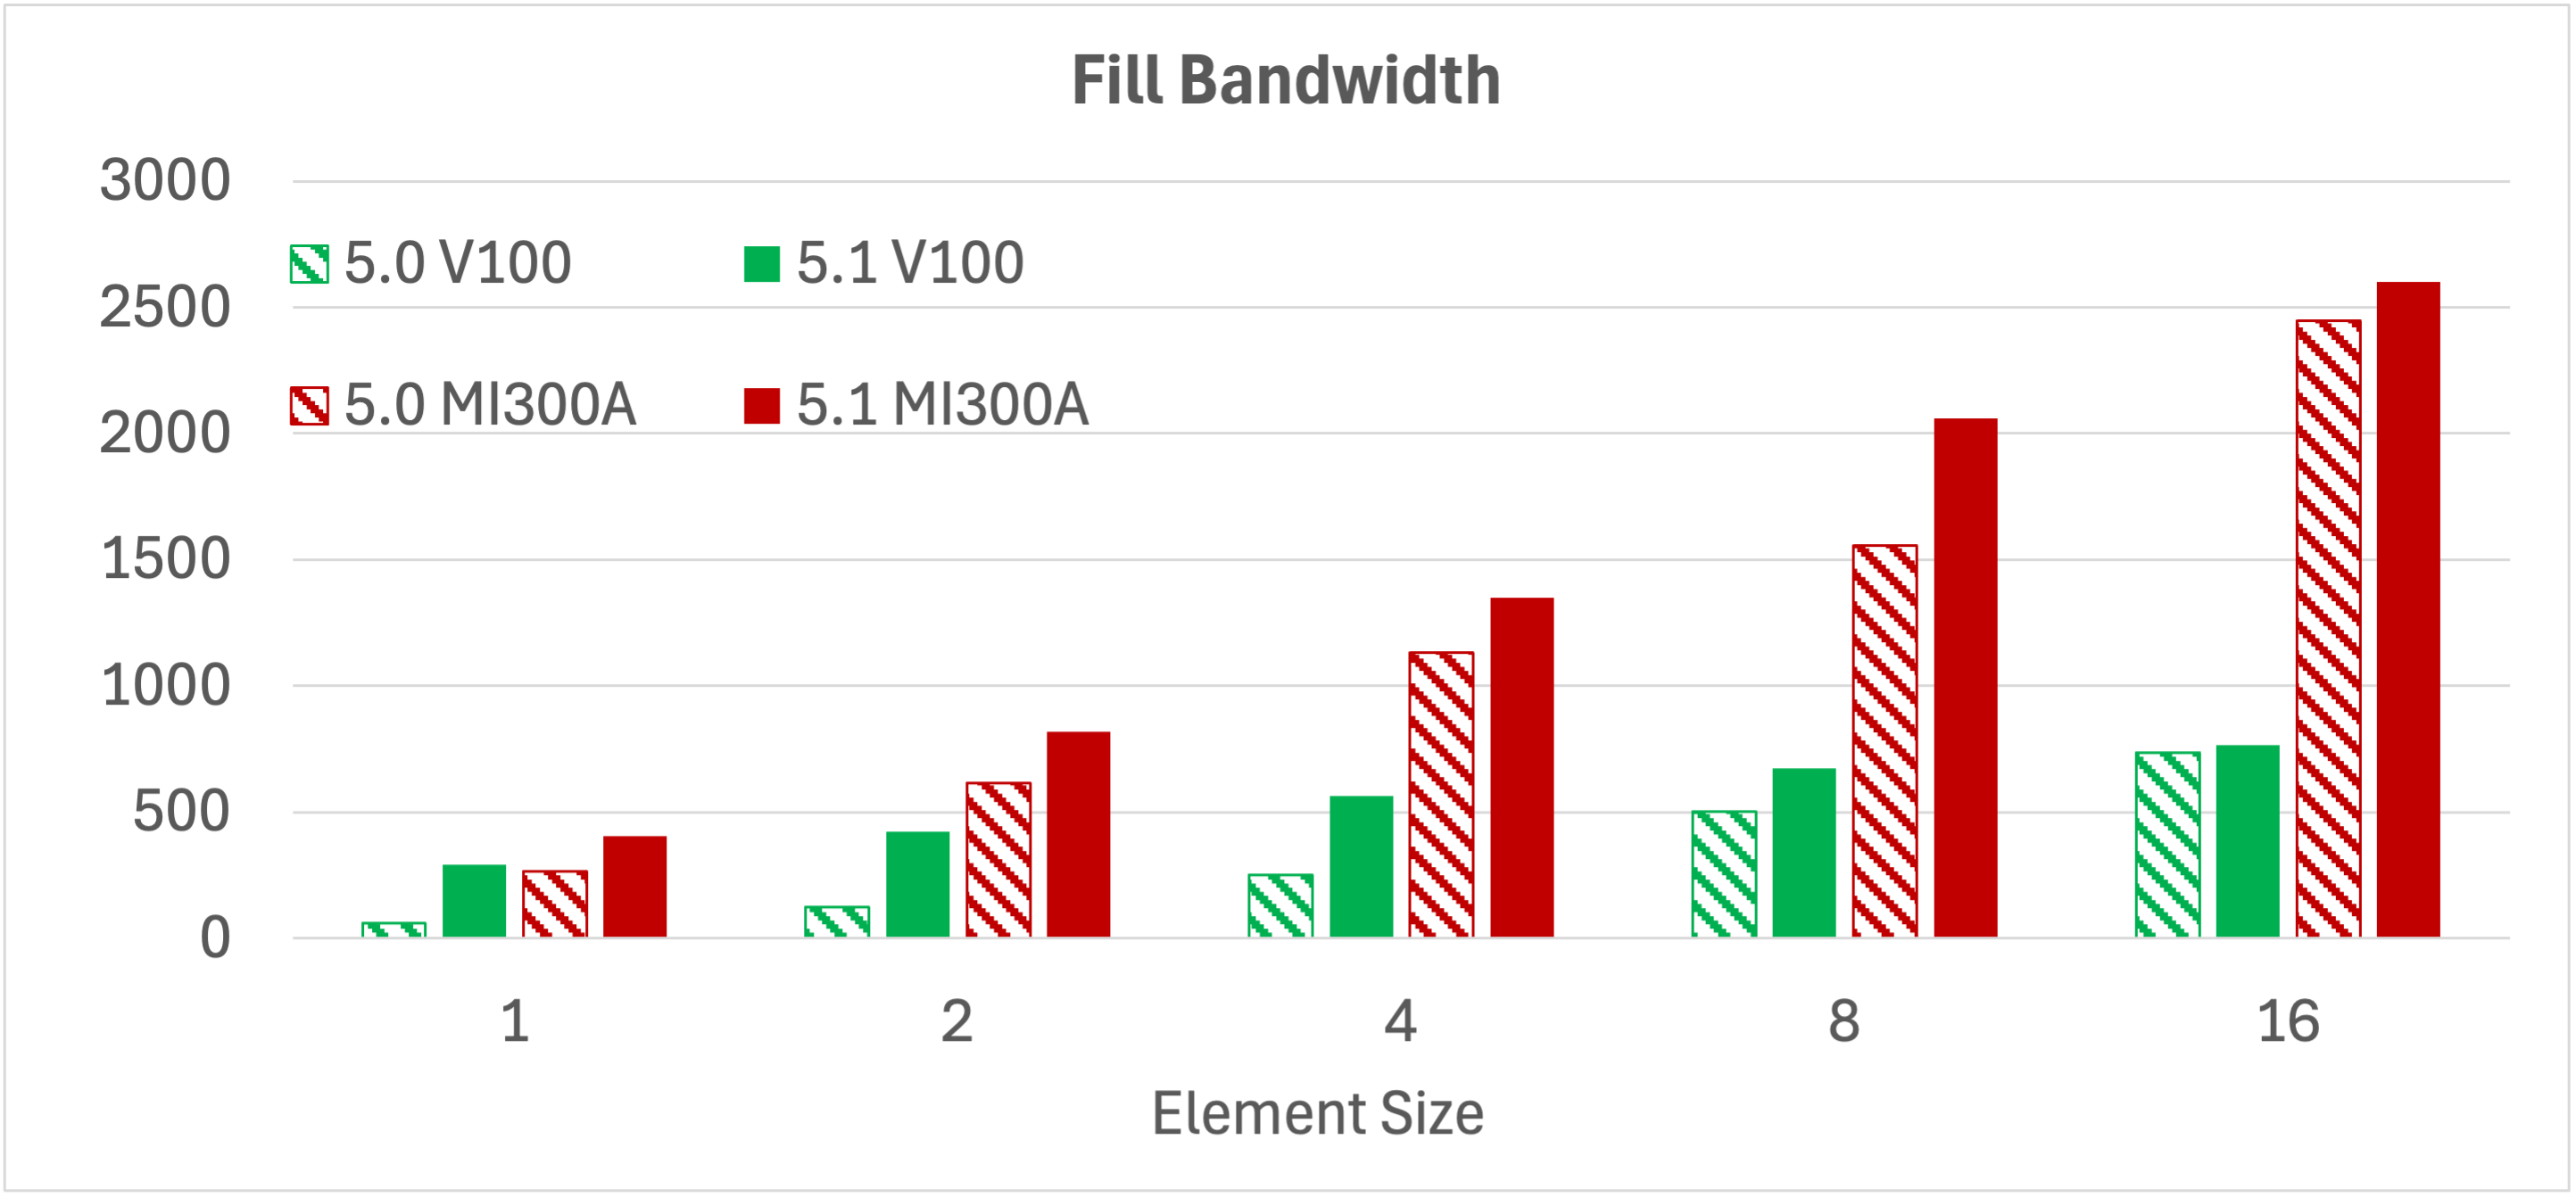
\includegraphics[width=0.5\textwidth]{5_1/fill-bandwidth.png}
\end{center}
\end{frame}

%==========================================================================

\begin{frame}[fragile]{General Enhancements II}
  \begin{itemize}
    \item Enforce failure when exceeding \texttt{team\_size\_max} and \texttt{scratch\_size\_max} checks
    \item Enable MPI detection with PALS
    \item Add \texttt{Kokkos::norm} for \texttt{Kokkos::complex} similar to \texttt{std::norm}
  \end{itemize}
\end{frame}

%==========================================================================

\begin{frame}[fragile]{Array Update}

  Relaxed constraints on \texttt{Kokkos::Array} subscript operator

  \vspace{1em}

  \begin{itemize}
    \item Previously, the indexer type was constrained so that the following holds:
    \begin{code}
      std::is_integral_v<IndexType> || std::is_enum_v<IndexType>
    \end{code}
    \item Now, only requires to be implictly convertible to \texttt{Kokkos::Array::size\_type}
  \end{itemize}

  \vspace{1.5em}

  This relaxation allows custom type indexers\\
  This is closer to the indexer constraints in \texttt{Kokkos::View}

\end{frame}

%==========================================================================

\begin{frame}[fragile]{Expand math support}
  Increase \texttt{\textbf{half}} and \texttt{\textbf{bhalf}} support
  \begin{itemize}
    \item Add \texttt{denorm\_min} traits
    \item Add non standard \texttt{rcp}, \texttt{rcpf} and \texttt{rcpl} functions.
    \item Extend \texttt{rsqrt} to half types
  \end{itemize}

\end{frame}

%==========================================================================

\begin{frame}[fragile]{Expand math support}
  Implement all remaining math functions
  \begin{itemize}
    \item Add \texttt{modf}, \texttt{modff} and \texttt{modfl} functions
    \item Add mathematical functions \texttt{frexp} \texttt{ldexp}, \texttt{scalbn}, \texttt{scalbln}
    \item Provide more quadruple precision floating-point manipulation functions.
    \item Add \texttt{isnormal} function for all floating-point types.
    \item Add binary predicate math comparison functions.
    \item Add fpclassify function.
    \item Round to integer math functions \texttt{rint} and \texttt{round}.
    \item Add std \texttt{nexttoward} wrapper.
  \end{itemize}

\end{frame}

%==========================================================================

\begin{frame}[fragile]{SIMD Enhancements}
  \begin{itemize}
    \item Added bitwise operators to all simd masks and simd vectors of integral types
    \begin{itemize}
      \item Bitwise ops: \texttt{\textasciitilde{}, \&{}, |, \^{}, \&=, |=, \^{}=}
    \end{itemize}

    \vspace{1em}

    \item Added simd memory permute functions
    \begin{itemize}
      \item \texttt{[unchecked|partial]\_gather\_from(in, indices, simd\_flag)}
      \item \texttt{[unchecked|partial]\_scatter\_to(simd, out, indices, simd\_flag)}
      \item Replace memory permute functions in deprecated \texttt{where\_expression}
    \end{itemize}
  \end{itemize}
\end{frame}

